\section{Introduction}\label{sec:intro}

AI data centers are adding on-site gas generation next to their IT load. The heat that remains
after power generation is low grade. A published dataset of a leadership supercomputer reports an
electricity draw of 8 to 30 MW and a waste-heat temperature of 30 to 38\,$^\circ$C
\citep{sun2024frontier}; a study of the same dataset lists typical coolant supply temperatures of
18 to 25\,$^\circ$C, return temperatures of 25 to 40\,$^\circ$C and 5 to 25 MW of heat
\citep{jadhav2026frontierml}. Combined heat and power has been proposed for data centers for some
time \citep{darrow2009chp}, and a single-effect absorption chiller can turn engine or turbine heat
into chilled water, at a measured coefficient of performance of 0.55 to 0.70 for one tested unit
\citep{ochoa2019absorption}. What a plant should look like for a given site, whether a plant model
is consistent, and where its exergy is lost are questions that need a thermodynamics expert.

Language models are a candidate assistant for these questions, and thermodynamics is a hard case
for them. ThermoQA is a benchmark built to measure thermodynamic reasoning in language models
\citep{duzkar2026thermoqa}, and in a study of gas-path analysis, smaller models struggled with tool
use and with extracting parameters \citep{song2024gaspath}. We do not measure general-purpose models
in this paper. Our concern is a failure that makes the problem worse: a plant model can solve, pass
range checks and still violate the second law, and nothing in the text of the model reveals it.
To our knowledge from the literature we reviewed (\cref{sec:related}), no verifiable environment
exists for the energy systems of data centers in which an answer is accepted only if it passes
mass, energy and exergy balances.

\paragraph{Idea.}
A physics simulator and a set of second-law verifiers form an environment whose checks are an
exact, cheap and verifiable reward. A small open model, Qwen3.5-4B \citep{qwen2026qwen35}, is to be
trained in two stages: LoRA supervised fine-tuning \citep{hu2021lora} on expert answers written
programmatically from the ground truth, then GRPO \citep{shao2024deepseekmath} against the
verifiers. The model formulates and diagnoses; the solver and the verifiers judge. \Cref{fig:fig_overview}
shows the system.

\begin{figure}[tbp]
\centering
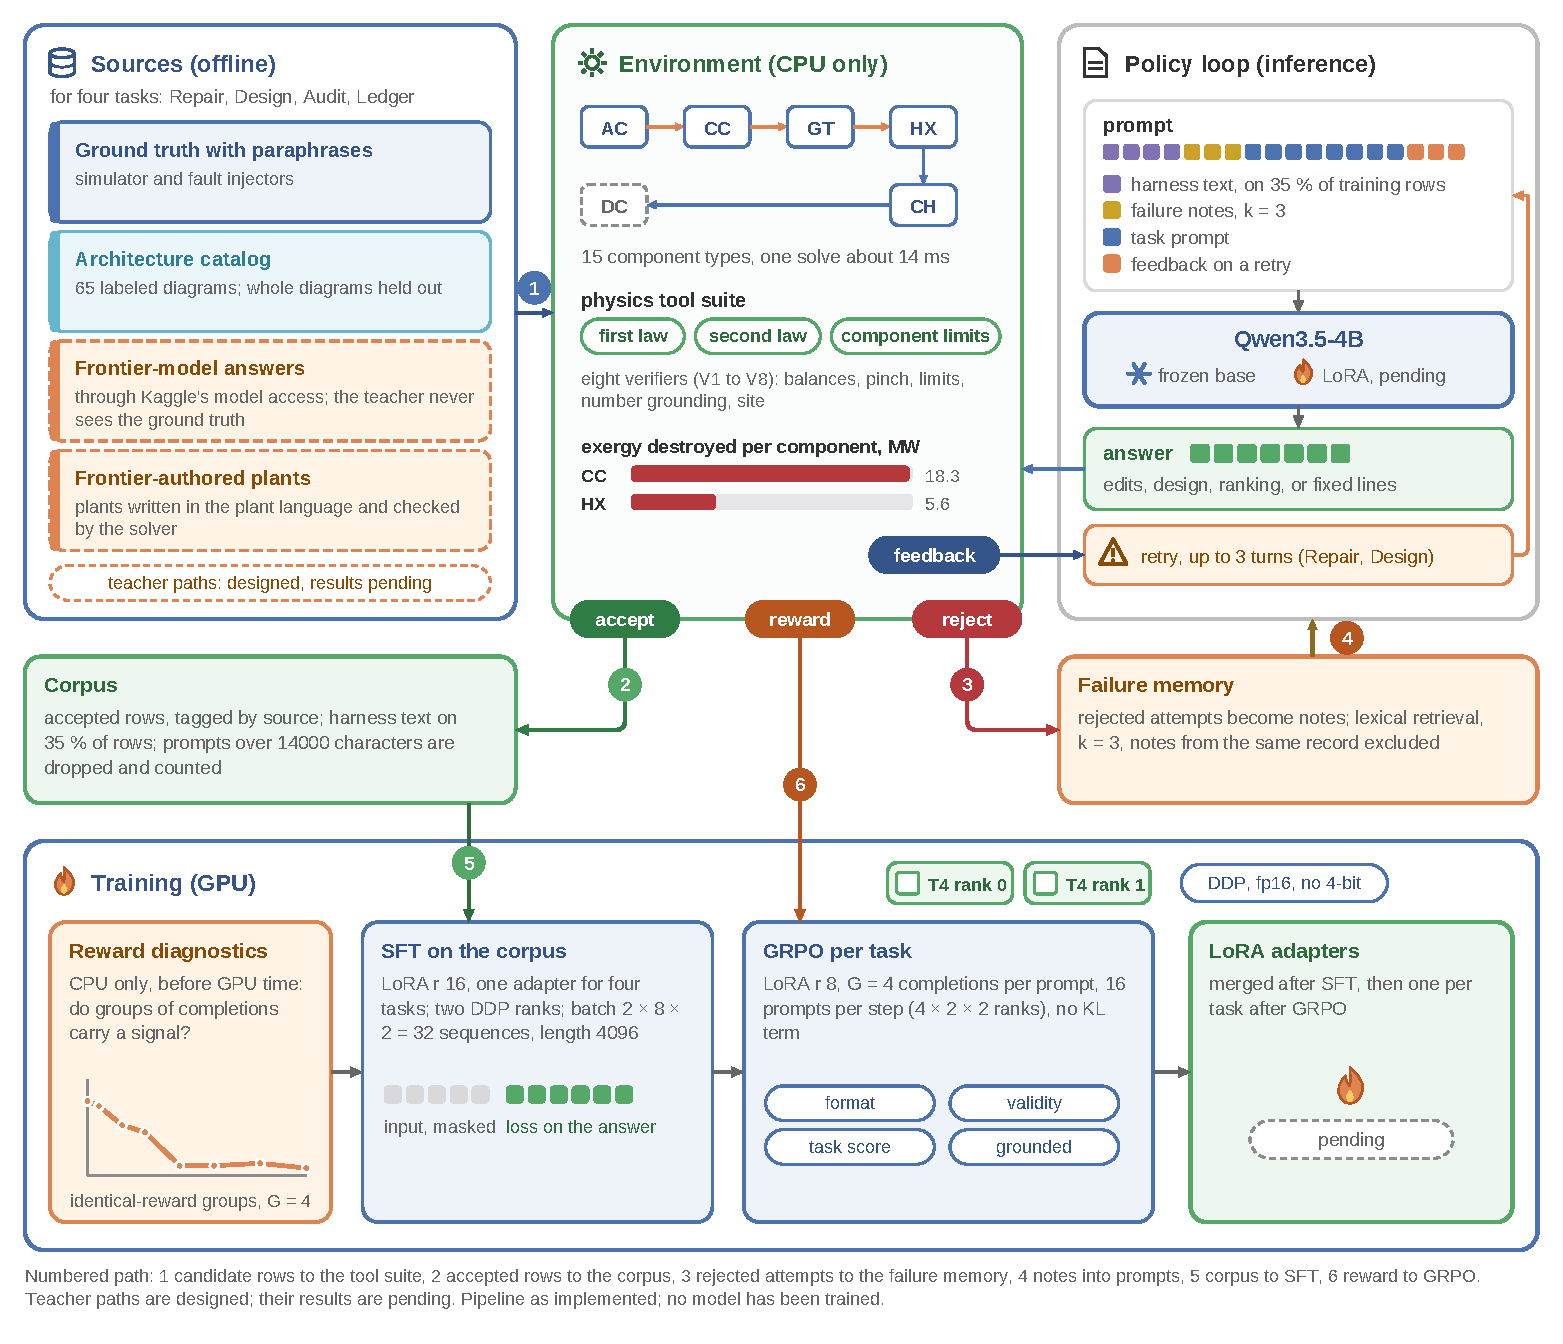
\includegraphics[width=\linewidth]{figures/pdf/fig_overview.pdf}
\caption{System overview. Offline, sampled plants, faults and a reference search give verified
expert answers for supervised fine-tuning and the reward for GRPO. The environment (simulator,
exergy accounting, verifiers V1 to V8) supplies the reward in training and the feedback at inference;
online, the model proposes an answer, the solver and the verifiers check it, and the model retries.
The figure shows the design, not results: no model has been trained, and every trained-model
statement is marked pending.}
\label{fig:fig_overview}
\end{figure}

\paragraph{Contributions.}
\begin{enumerate}[leftmargin=*,itemsep=2pt]
\item A second-law-verified environment for data-center energy systems: \val{env.n_components}
component models, exergy accounting against an explicit dead state, and verifiers V1 to V8
whose checks are the reward (\cref{sec:method}).
\item Four task families with structural out-of-distribution splits: Repair (parameter-level faults,
\val{env.n_repair_faults} types), Design (a catalog of \val{env.n_catalog} configurations,
\val{env.n_catalog_heat} when there is a heat demand, plus continuous parameters), Audit (rank
exergy destroyers, propose one allowed change, predict its fuel effect) and Ledger repair
(\val{env.n_ledger_faults} equation-level fault types in an exergy ledger, which range checks cannot
see).
\item An evaluation that counts solver calls: non-model baselines, an anytime protocol for sample
efficiency, paired statistics, and ablations that include an agent harness (an \texttt{AGENTS.md}
file plus generated skills) with a held-out component.
\item Simulator findings that do not depend on a model: feasibility limits of the catalog, first-law
against second-law blame, the symptom coverage of equation faults, and trace and modular-fleet bounds
(\cref{sec:experiments,sec:trace}).
\end{enumerate}

\paragraph{What we do not claim.}
We do not claim that a trained model beats numerical optimization on the final optimum for a fixed
superstructure. We do not claim any validation against a real plant, and there is no measured
on-site-generation data center in this work: measured load and coolant traces from published data
set the operating points of a physics model, and all training data is synthetic. No model has been
trained, so we make no claim about trained-model results; for the trained model we intend to claim
only sample efficiency and breadth, and only once the pending runs exist.

\paragraph{Paper map.}
\Cref{sec:related} places the work among related studies. \Cref{sec:method} describes the
environment, the verifiers, the tasks, the rewards, the training recipe and the agent harness.
\Cref{sec:experiments} states the frozen evaluation protocol, reports the non-model baselines and
simulator findings that were measured, and gives the skeletons of the pending model results.
\Cref{sec:trace} covers trace and fleet bounds, \cref{sec:limits} lists the limits, and the appendix
holds definitions, registries and the reproduction recipe.
